\documentclass[11pt]{opticajnl}
\journal{opticajournal} 

\setboolean{shortarticle}{true}


\usepackage{lineno}
\usepackage{multicol}
\usepackage{tabularray}
\usepackage{pdfpages}  
\usepackage{listings}
\usepackage{tikz}
\usepackage{xcolor}  
\definecolor{crimson}{HTML}{ca3142}
\lstdefinestyle{terminal}{
  backgroundcolor=\color{white},   % Fondo blanco
  basicstyle=\color{black}\ttfamily, % Texto negro en fuente monoespaciada
  keywordstyle=\color{blue}\bfseries, % Palabras clave en azul y negrita
  commentstyle=\color{green!70}\ttfamily, % Comentarios en verde
  stringstyle=\color{red}\ttfamily, % Cadenas en rojo
  morekeywords={sudo, apt-get, install, cd, ls, mkdir, rm, rmdir, cp, mv, echo, cat, nano, vim, grep, find, chmod, chown, systemctl, service, update, upgrade, reboot, shutdown, exit}, % Comandos comunes de terminal
  breaklines=true, % Permitir saltos de línea
  frame=single, % Marco alrededor del código
  framerule=0.5pt, % Grosor del marco
  rulecolor=\color{gray}, % Color del marco
  xleftmargin=0.05\textwidth, % Margen izquierdo
  xrightmargin=0.05\textwidth, % Margen derecho
  aboveskip=1em, % Espacio antes del bloque de código
  belowskip=1em % Espacio después del bloque de código
}

\lstdefinestyle{sql}{
  language=SQL,
  showspaces=false, 
  basicstyle=\ttfamily,
  numbers=left,
  numberstyle=\tiny,
  backgroundcolor=\color{gray!10},
  keywordstyle=\color{blue}\bfseries,
  commentstyle=\color{green!70}\ttfamily,
  stringstyle=\color{red!70}\ttfamily,
  breaklines=true,
  morekeywords={CREATE, DROP, TABLE, SELECT, INSERT, UPDATE, DELETE, FROM, WHERE, JOIN, ON, AS}, % Puedes añadir más palabras clave específicas de SQL.
  literate={``}{``}1 {''}{''}1 {“}{``}1 {”}{''}1 {‘}{`}1 {’}{'}1
}

%\linenumbers % Turn off line numbering for Optica Open preprint submissions.

\title{El Guachinche}

%\author[1,2,3]{Luis Ardévol Mesa, Carlos Martínez García \\ \copyrightstatement}
\author[1,2,3]{Luis Ardévol Mesa, Carlos Martínez García, Miguel Mato Martínez}

\begin{document}

\begin{titlepage}
\begin{center}
    \vspace*{5cm}
    
    {\huge\bfseries El Guachinche\par}
    \vspace{1cm}
    
    {\Large\color{crimson} Proyecto de Inteligencia de Negocio\par}
    \vspace{1cm}
    
    
\begin{tikzpicture}
    \draw[thick, color=crimson] (0,0) -- (8,0);
    \end{tikzpicture}
    
    \vspace{1.5cm}
    {\large Luis Ardévol Mesa\\
    Carlos Martínez García\\
    Miguel Mato Martínez\par}
    
    \vfill
    
    {\large Proyecto Final de Prácticas\par}
    
    \vspace{2cm}
    
    {\large Diciembre, 2024\par}
\end{center}
\end{titlepage}

\maketitle

\setcounter{tocdepth}{2}
\tableofcontents

\hrulefill

\section{Introducción}

Los \textit{guachinches} son establecimientos (en la propia vivienda del propietario) que surgen en la zona del norte de Tenerife como solución para vender el excedente de vino de cada cosecha. El vino se acompaña típicamente con platos tradicionales de la cocina canaria. Actualmente, según el Decreto 83/2013\footnote{\url{https://www.gobiernodecanarias.org/boc/2013/153/001.html}}, hay una regulación muy estricta amparando a estos locales y al viticultor; muchos establecimientos comúnmente denominados ``guachinches'', entran dentro de la categoría \textit{restaurante}, al salirse de lo establecido en este decreto. \\

El Guachinche nace de una idea sencilla pero atractiva: traer el espíritu de los tradicionales guachinches canarios al resto de España, pero con un toque especial. En nuestra cocina, las recetas isleñas comparten protagonismo con una cuidada selección de arepas para todos los públicos, todo esto acompañado de los mejores vinos de las Islas. Es ese equilibrio entre tradición y adaptación lo que nos hace únicos: cada local incorpora platos de la región, porque creemos que la gastronomía local es parte fundamental de nuestra historia. \\

No obstante, quien entra a El Guachinche no solo viene a comer. Para dar una experiencia lo más cercana posible y crear una atmósfera atractiva y familiar para los comensales, nuestros locales presentan una ambientación tradicional y hogareña. La experiencia no sería completa de no ser por nuestro personal, siempre cercano. \\

Actualmente, El Guanchinche cuenta con 13 locales, repartidos en Canarias (7), Galicia (2), Andalucía (2) y Comunidad Valenciana (2). El crecimiento en los últimos dos años ha sido exponencial, por lo que desde la dirección de la empresa nos vemos en la necesidad de implementar un modelo de inteligencia de negocio que nos permita tomar decisiones basadas en datos, priorizando siempre al cliente. \\

\noindent Los objetivos principales perseguidos por la cadena son los siguientes: 
\begin{itemize}
\item Fidelización de clientes. En esta línea, sería conveniente que la economía de cada local no dependiera de la nueva clientela, ya que la fuente de ingresos sería menos estable. 
\item Mejorar la experiencia general del cliente en nuestros locales. 
\item Adaptar la oferta gastronómica a las preferencias de cada región.
\item Ampliar beneficios, especialmente en las regiones menos rentables actualmente.
\item Estudio de la rentabilidad del servicio a domicilio.
\end{itemize}

El servicio a domicilio corre a cargo de dos empresas: Uber Eats y Glovo. Conocida la comisión de estos servicios, cada local descuenta esta comisión del total y almacena el beneficio real de cada pedido a domicilio. Para cumplir con los objetivos, es importante conocer: 
\begin{itemize}
\item La cantidad de nuevos clientes en comparación a los habituales. 
\item La satisfacción de los clientes con los servicios prestados en nuestros establecimientos.
\item El rendimiento económico de cada uno de los locales, así como de la totalidad de la cadena. Esto incluye:
\begin{itemize}
\item Ventas de cada producto ofertado.
\item Gastos e ingresos de cada local. En estos últimos sería necesario distinguir entre ingresos presenciales e ingresos a domicilio. 
\end{itemize}
\end{itemize}

A continuación, se describen los procesos de diseño y construcción del almacén de datos para gestionar la información necesaria. Posteriormente, se comentarán los procesos de extracción, transformación y carga que permiten la creación y actualización del almacén de datos. Se sigue con algunas consultas de interés para los objetivos descritos anteriormente y, para terminar, se incluyen cuadros de mando e informes adecuados al caso de estudio. Todos los archivos usados y generados se encuentran a disposición en el siguiente repositorio: \href{https://github.com/uisitoam/El-Guachinche}{\texttt{https://github.com/uisitoam/El-Guachinche}}

\section{Diseño y construcción del almacén de datos}

Nuestros locales llevan un registro cuidadoso de los aspectos más importantes de la actividad diaria, como son las ventas, los gastos o la opinión de los clientes. Cada local genera reportes mensuales que recogen estos datos y son enviados a la central para su análisis. Estos reportes son los que nos permitirán obtener la información necesaria para la toma de decisiones. 

\subsection{Diseño del almacén de datos}

Para mostrar el diseño del almacén de datos, es necesario describir primero la estructura de los datos recogidos en los reportes de cada local. Concretamente, cada mes se reciben dos archivos de datos por cada local de nuestra cadena. El primero de ellos contiene toda la información relacionada con la economía del restaurante: desglose de gastos en cuatro categorías (personal, suministros, alquiler y otros), ingresos por ventas (diferenciando entre los servicios presencial y domicilio) y clientela. Esto será beneficio para varios de los objetivos de la cadena. Siendo un poco más específicos, se proporcionan los siguientes datos:
\begin{itemize}
\item Un identificador entero para cada local, generado por la central en orden de apertura.
\item La fecha de envío del reporte (establecida para el primer día del mes). 
\item Los gastos en alquiler, personal, suministros (proveedores), y extras (limpieza, mantenimiento, etc.), todo en euros.
\item Los ingresos, tanto por vía presencial como a domicilio, en euros. Como ya se ha mencionado, estos ingresos ya tienen descontada la comisión de Uber Eats o Glovo.
\item Los clientes totales por ambos canales, así como el número de clientes nuevos.
\item Los platos ofertados en el local, cada uno con los siguientes datos:
\begin{itemize}
\item Un identificador entero para cada plato, generado por la central.
\item El nombre, precio y número de ventas del plato. 
\end{itemize}
\end{itemize}

Estos datos se recogen en un archivo XML como el que se muestra en la figura \ref{fig:xml_economico}.

\begin{figure}[h]
\centering
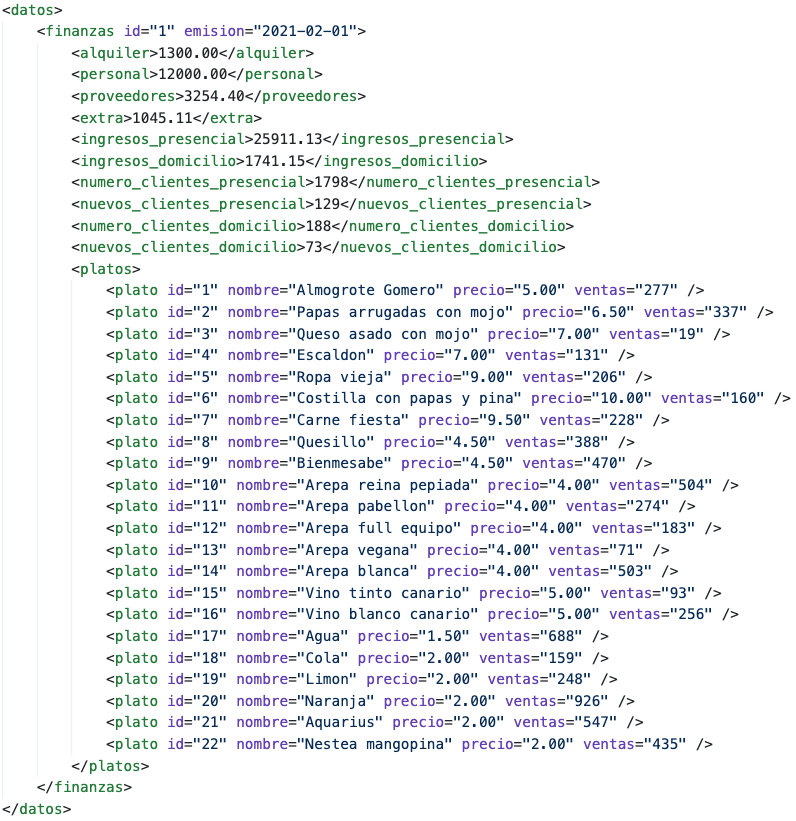
\includegraphics[width=0.6\textwidth]{fotos/1.png}
\caption{Ejemplo de archivo XML con los datos económicos mensuales de un local.}
\label{fig:xml_economico}
\end{figure}

\noindent Los identificadores de los locales son los siguientes:
\begin{multicols}{2}
\begin{itemize}
\item 1: La Laguna, Tenerife.
\item 2: Hermigua, La Gomera.
\item 3: Cotillo, Fuerteventura.
\item 4: Las Palmas de Gran Canaria, Gran Canaria.
\item 5: Tazacorte, La Palma.
\item 6: Valverde, El Hierro.
\item 7: Arrecife, Lanzarote.
\item 8: Granada, Granada.
\item 9: Sevilla, Sevilla.
\item 10: Santiago de Compostela, A Coruña.
\item 11: Vigo, Pontevedra.
\item 12: Alicante, Comunidad Valenciana.
\item 13: Valencia, Comunidad Valenciana. 
\end{itemize}
\end{multicols}

\noindent Los identificadores de los productos son los siguientes:
\begin{multicols}{3}
\begin{itemize}
\item 1: Almogrote Gomero.
\item 2: Papas arrugadas con mojo.
\item 3: Queso asado con mojo.
\item 4: Escaldón.
\item 5: Ropa vieja.
\item 6: Costilla con papas y piña.
\item 7: Carne fiesta.
\item 8: Quesillo.
\item 9: Bienmesabe.
\item 10: Arepa reina pepiada.
\item 11: Arepa pabellón.
\item 12: Arepa full equipo.
\item 13: Arepa vegana.
\item 14: Arepa blanca.
\item 15: Vino tinto canario.
\item 16: Vino blanco canario.
\item 17: Agua.
\item 18: Refresco de cola.
\item 19: Refresco de limón.
\item 20: Refresco de naranja.
\item 21: Aquarius.
\item 22: Nestea mango-piña.
\item 23: Salmorejo.
\item 24: Pescaito frito.
\item 25: Gambitas de Huelva.
\item 26: Pestiños.
\item 27: Vino tinto andaluz.
\item 28: Vino blanco andaluz.
\item 29: Pulpo a feira.
\item 30: Empanada (porción).
\item 31: Lacon con grelos.
\item 32: Tarta de Santiago.
\item 33: Vino tinto gallego.
\item 34: Vino blanco gallego.
\item 35: Paella.
\item 36: Arroz negro.
\item 37: Esgarraet. 
\item 38: Fartons. 
\item 39: Vino tinto valenciano.
\item 40: Vino blanco valenciano.
\end{itemize}
\end{multicols}

Como bien describe el objetivo del negocio, cada región tiene sus platos típicos. Los 22 primeros productos son comunes a todos los locales de la cadena, mientras que a partir de ahí, cada región incorpora distintos productos, como es el caso del \textit{salmorejo} en Andalucía, el \textit{lacçon con grelos} en Galicia o el \textit{esgarraet} en la Comunidad Valenciana. Así mismo, cada local ofrece vinos de proximidad. \\

Para cumplir los objetivos relacionados con la satisfacción y fidelización de clientes, cada local proporciona un segundo archivo, en este caso en formato CSV, con valoraciones de los clientes: en caso de ser clientes presenciales, se valora el ambiente del local, el personal y la calidad de la comida, mientras que los clientes a domicilio simplemente hacen llegar una valoración del servicio general. Así, cada fila del archivo da el identificador del local, la fecha de la valoración, y las votaciones correspondientes (3 en el caso de clientes presenciales, una en el caso de clientes a domicilio). Un ejemplo de este archivo se muestra en la figura \ref{fig:csv_valoraciones}.

\begin{figure}[h]
\centering
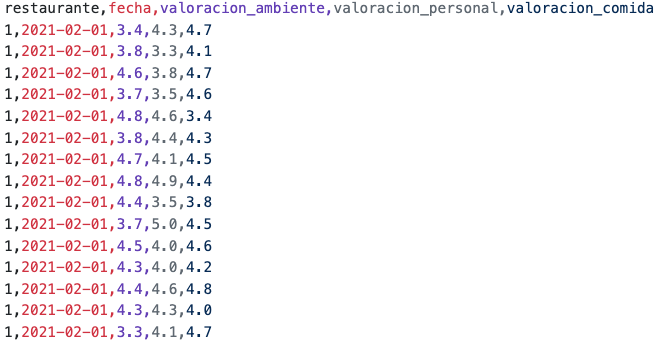
\includegraphics[width=0.6\textwidth]{fotos/2.png}
\caption{Ejemplo de archivo CSV con las valoraciones de los clientes de un local.}
\label{fig:csv_valoraciones}
\end{figure}

Se dará a los datos almacenados de cada uno de los archivos anteriores la máxima granularidad posible, es decir, mensual. Las dimensiones seleccionadas son las siguientes:
\begin{itemize}
\item \textbf{Tiempo}: la dimensión temporal de los datos se representa mediante dos niveles: año y mes.
\item \textbf{Restaurante}: la dimensión restaurante actúa como dimensión geográfica. Se tendrán en cuenta todos los locales de la cadena y se mostrarán dos niveles, uno para el país y otro para la ciudad.
\item \textbf{Producto}: la dimensión producto recoge todos los platos ofertados en los locales de la cadena. Esta es una dimensión plana que muestra los productos y el precio asociado a cada uno de ellos.
\end{itemize}
\noindent Los hechos seleccionados para el almacén de datos son los siguientes:
\begin{itemize}
\item \textbf{Finanzas}: se almacenan los costes e ingresos de los locales, junto con los datos de los clientes para cada combinación de las siguientes dimensiones: tiempo (mes de envío de los reportes) y restaurante (mediante el identificador de cada local).
\item \textbf{Producto}: se almacenan los hechos relacionados con las ventas de los productos ofertados en los locales, para cada combinación de las siguientes dimensiones: tiempo (mes de envío de los reportes), restaurante (mediante el identificador de cada local) y producto (mediante el identificador de cada plato). Se tiene el númer ototal de ventas mensuales de un producto, así como un cálculo de los ingresos generados por ese producto, a partir de sus ventas y su precio.
\item \textbf{Feedback}: se almacenan las valoraciones de los clientes para cada combinación de las siguientes dimensiones: tiempo (mes de envío de los reportes) y restaurante (mediante el identificador de cada local). Se almacena la media de las valoraciones de los clientes para cada uno de los aspectos recogidos en los reportes.
\end{itemize}

Por tanto, el modelo conceptual del almacén de datos se muestra en la figura \ref{fig:esquema_almacen}, siendo un esquema con tres estrellas y tres dimensiones. \\

\begin{figure}[h]
\centering
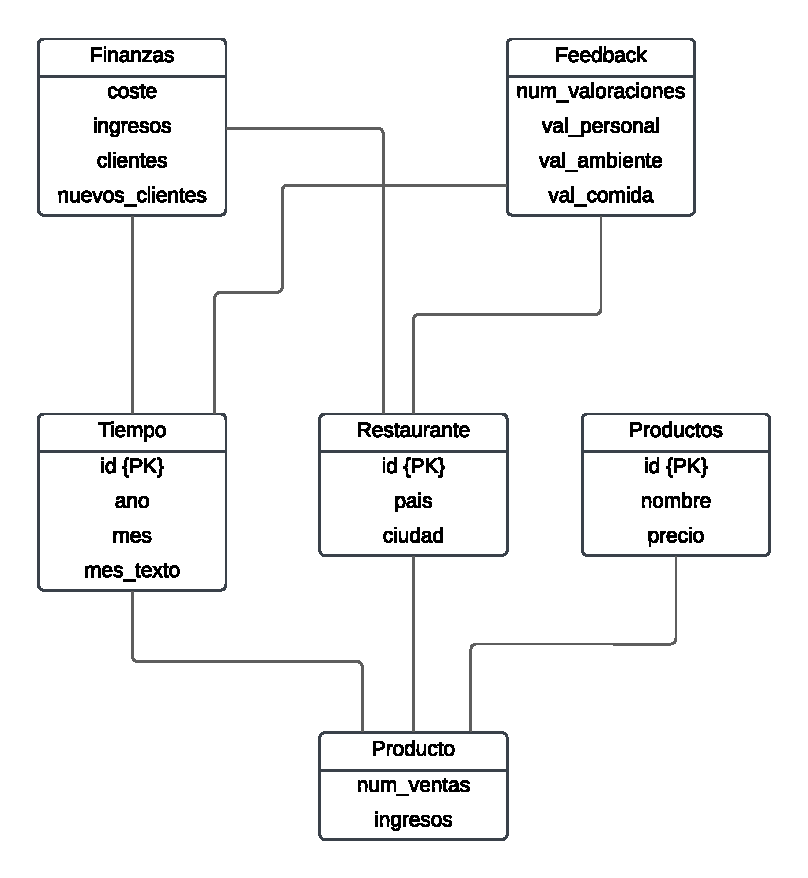
\includegraphics[width=0.7\textwidth]{fotos/3.pdf}
\caption{Esquema conceptual del almacén de datos.}
\label{fig:esquema_almacen}
\end{figure}

\noindent Los detalles de la implementación del almacén de datos se describen en las siguientes tablas: 

\newpage

\begin{longtblr}[
    caption = {Descripción de las dimensiones del almacén de datos.},
    label = {tab:modelo-datos}
]{
    colspec = {p{3.75cm}p{1.75cm}X},
}
% Dimensiones
& & \\\hline\hline
\SetCell[c=3]{c, h} Tiempo \\\hline\hline
\SetCell{c} Atributo & \SetCell{c} Tipo & \SetCell{c} Descripción \\ \hline
\SetCell{l} id (pk) & Integer & Identificador autoincremental generado por el almacén cada vez que se inserta un nuevo mes. \\ \hline
\SetCell{l} ano & Integer & Número correspondiente al año. \\ \hline
\SetCell{l} mes & Integer & Número correspondiente al mes dentro del año. \\ \hline
\SetCell{l} mes\_texto & String & Texto con el nombre del mes. \\ \hline
& & \\ 
& & \\ 
& & \\ 
& & \\ \hline\hline
\SetCell[c=3]{c} Restaurante \\ \hline\hline
\SetCell{c} Atributo & \SetCell{c} Tipo & \SetCell{c} Descripción \\ \hline
\SetCell{l} id (pk) & Integer & Identificador de cada local, generado por la central. \\ \hline
\SetCell{l} pais & String & País donde se sitúa el local. \\ \hline
\SetCell{l} ciudad & String & Ciudad donde se sitúa el local. \\ \hline
& & \\ 
& & \\ \hline\hline
\SetCell[c=3]{c} Producto \\ \hline\hline
\SetCell{c} Atributo & \SetCell{c} Tipo & \SetCell{c} Descripción \\ \hline
\SetCell{l} id (pk) & Integer & Identificador de cada plato, generado por la central. \\ \hline
\SetCell{l} nombre & String & Nombre del plato. \\ \hline
\SetCell{l} precio & Numeric & Precio del plato. \\ \hline
\end{longtblr}

\begin{longtblr}[
    caption = {Descripción de los hechos del almacén de datos.},
    label = {tab:modelo-datos2}
]{
    colspec = {p{3.75cm}p{1.75cm}X},
}
% Hechos
& & \\ 
\hline\hline
\SetCell[c=3]{c} Finanzas \\ \hline\hline
\SetCell{c} Atributo & \SetCell{c} Tipo & \SetCell{c} Descripción \\ \hline
\SetCell{l} alquiler & Numeric & Gasto en alquiler de un local, en euros. \\ \hline
\SetCell{l} personal & Numeric & Gasto en personal de un local, en euros. \\ \hline
\SetCell{l} proveedores & Numeric & Gasto en suministros de un local, en euros. \\ \hline
\SetCell{l} extra & Numeric & Gasto en extras de un local, en euros. \\ \hline
\SetCell{l} ingresos\_presencial & Numeric & Ingresos por ventas presenciales de un local, en euros. \\ \hline
\SetCell{l} ingresos\_domicilio & Numeric & Ingresos por ventas a domicilio de un local, en euros. \\ \hline
\SetCell{l} numero\_clientes\_ presencial & Integer & Número total de clientes presenciales de un local. \\ \hline
\SetCell{l} numero\_clientes\_ domicilio & Integer & Número total de clientes a domicilio de un local. \\ \hline
\SetCell{l} nuevos\_clientes\_ presencial & Integer & Número de clientes presenciales nuevos de un local. \\ \hline
\SetCell{l} nuevos\_clientes\_ domicilio & Integer & Número de clientes nuevos a domicilio de un local. \\ \hline
& & \\ 
& & \\ 
& & \\ 
& & \\ \hline\hline
\SetCell[c=3]{c} Producto (Ventas) \\ \hline\hline
\SetCell{c} Atributo & \SetCell{c} Tipo & \SetCell{c} Descripción \\ \hline
\SetCell{l} ventas & Integer & Número total de ventas de un producto en un local. \\\hline 
\SetCell{l} ingresos & Numeric & Ingresos totates de un producto en un local. \\\hline 
& & \\ 
& & \\ \hline\hline
\SetCell[c=3]{c} Feedback \\ \hline\hline
\SetCell{c} Atributo & \SetCell{c} Tipo & \SetCell{c} Descripción \\ \hline
\SetCell{l} valoracion\_ambiente & Numeric & Valoración promedio (entre 0 y 5 con un decimal) del ambiente de un local, según sus clientes. \\ \hline
\SetCell{l} valoracion\_personal & Numeric & Valoración promedio (entre 0 y 5 con un decimal) del personal de un local, según sus clientes. \\ \hline
\SetCell{l} valoracion\_comida & Numeric & Valoración promedio (entre 0 y 5 con un decimal) de la calidad de la comida de un local, según sus clientes. \\ \hline
\end{longtblr}










\subsection{Creación de los cubos de datos}

Utilizando como base las estructuras de datos relacionales descritas en el apartado anterior, se crea un esquema multidimensional con tres cubos y tres dimensiones compartidas entre ellos. Estas se definen a nivel de esquema y posteriormente se reutilizan a nivel de cubo:

\begin{itemize}
\item Dimensión: \textbf{Tiempo}. Dimensión de tipo temporal.
\begin{itemize}
\item Jerarquía: \textit{jerarquiaTiempo}. Definida por el atributo \textit{id}. 
\begin{itemize}
\item Nivel: \textit{ano}. Nivel de tipo \textit{TimeYears} definido por el atributo \textit{ano}.
\item Nivel: \textit{mes}. Nivel de tipo \textit{TimeMonths} definido por el atributo \textit{mes}. Se utiliza el atributo \textit{mes\_texto} para nombrar a los elementos de este nivel.
\item Tabla: tiempo
\end{itemize}
\end{itemize}
\item Dimensión: \textbf{Restaurante}. Dimensión de tipo estándar.
\begin{itemize}
\item Jerarquía: \textit{jerarquiaRestaurantes}. Definida por el atributo \textit{id}.
\begin{itemize}
\item Nivel: \textit{pais}. Nivel de tipo regular definido por el atributo \textit{pais}.
\item Nivel: \textit{ciudad}. Nivel de tipo regular definido por el atributo \textit{ciudad}.
\item Tabla: restaurante
\end{itemize}
\end{itemize}
\item Dimensión: \textbf{Productos}. Dimensión de tipo estándar.
\begin{itemize}
\item Jerarquía: \textit{jerarquiaProductos}. Definida por el atributo \textit{id}.
\begin{itemize}
\item Nivel: \textit{nombre}. Nivel de tipo regular definido por el atributo \textit{nombre}.
\item Tabla: producto
\end{itemize}
\end{itemize}
\item Cubo: \textbf{Finanzas}. 
\begin{itemize}
\item Tabla: \textit{finanzas}
\item Dimensiones 
\begin{itemize}
\item Dimensión usada: \textbf{Tiempo}. Se referencia a la dimensión \textit{Tiempo}. Se utiliza el atributo \textit{fecha} como clave foránea.
\item Dimensión usada: \textbf{Restaurante}. Se referencia a la dimensión \textit{Restaurante}. Se utiliza el atributo \textit{restaurante} como clave foránea.
\end{itemize}
\item Medidas
\begin{itemize}
\item Medida: \textbf{Alquiler}. Se agrega el atributo \textit{alquiler} usando la función SUM.
\item Medida: \textbf{Personal}. Se agrega el atributo \textit{personal} usando la función SUM.
\item Medida: \textbf{Proveedores}. Se agrega el atributo \textit{proveedores} usando la función SUM.
\item Medida: \textbf{Extra}. Se agrega el atributo \textit{extra} usando la función SUM.
\item Medida: \textbf{Ingresos presencial}. Se agrega el atributo \textit{ingresos\_presencial} usando la función SUM.
\item Medida: \textbf{Ingresos domicilio}. Se agrega el atributo \textit{ingresos\_domicilio} usando la función SUM.
\item Medida: \textbf{Número clientes presencial}. Se agrega el atributo \textit{numero\_clientes\_presencial} usando la función SUM.
\item Medida: \textbf{Número clientes domicilio}. Se agrega el atributo \textit{número\_clientes\_domicilio} usando la función SUM.
\item Medida: \textbf{Nuevos clientes presencial}. Se agrega el atributo \textit{nuevos\_clientes\_presencial} usando la función SUM.
\item Medida: \textbf{Nuevos clientes domicilio}. Se agrega el atributo \textit{nuevos\_clientes\_domicilio} usando la función SUM.
\item Medida calculada: \textbf{Gastos totales}. Se genera un nuevo valor para la dimensión \textit{Measures} usando la expresión MDX: ``[Measures].[Alquiler] + [Measures].[Personal] + [Measures].[Proveedores] + [Measures].[Extra]''
\item Medida calculada: \textbf{Ingresos totales}. Se genera un nuevo valor para la dimensión \textit{Measures} usando la expresión MDX: ``[Measures].[Ingresos presencial] + [Measures].[Ingresos domicilio]''
\item Medida calculada: \textbf{Beneficio}. Se genera un nuevo valor para la dimensión \textit{Measures} usando la expresión MDX: ``[Measures].[Ingresos totales] - [Measures].[Gastos totales]''
\item Medida calculada: \textbf{Número total clientes}. Se genera un nuevo valor para la dimensión \textit{Measures} usando la expresión MDX: ``[Measures].[Número clientes presencial] + [Measures].[Número clientes domicilio]''
\item Medida calculada: \textbf{Número total nuevos clientes}. Se genera un nuevo valor para la dimensión \textit{Measures} usando la expresión MDX: ``[Measures].[Nuevos clientes] + [Measures].[Nuevos clientes domicilio]''
\item Medida calculada: \textbf{Beneficio por cliente}. Se genera un nuevo valor para la dimensión \textit{Measures} usando la expresión MDX: ``[Measures].[Beneficio] / [Measures].[Número total clientes]''
\end{itemize}
\end{itemize}
\item Cubo: \textbf{Producto (Ventas)}.
\begin{itemize}
\item Tabla: \textit{producto}
\item Dimensiones
\begin{itemize}
\item Dimensión usada: \textbf{Tiempo}. Se referencia a la dimensión \textit{Tiempo}. Se utiliza el atributo \textit{fecha} como clave foránea.
\item Dimensión usada: \textbf{Restaurante}. Se referencia a la dimensión \textit{Restaurante}. Se utiliza el atributo \textit{restaurante} como clave foránea.
\item Dimensión usada: \textbf{Producto}. Se referencia a la dimensión \textit{Producto}. Se utiliza el atributo \textit{producto} como clave foránea.
\end{itemize}
\item Medidas
\begin{itemize}
\item Medida: \textbf{Ventas}. Se agrega el atributo \textit{ventas} usando la función SUM.
\end{itemize}
\end{itemize}
\item Cubo: \textbf{Feedback}.
\begin{itemize}
\item Tabla: \textit{feedback}
\item Dimensiones
\begin{itemize}
\item Dimensión usada: \textbf{Tiempo}. Se referencia a la dimensión \textit{Tiempo}. Se utiliza el atributo \textit{fecha} como clave foránea.
\item Dimensión usada: \textbf{Restaurante}. Se referencia a la dimensión \textit{Restaurante}. Se utiliza el atributo \textit{restaurante} como clave foránea.
\end{itemize}
\item Medidas
\begin{itemize}
\item Medida: \textbf{Valoración ambiente}. Se agrega el atributo \textit{valoracion\_ambiente} usando la funcion AVG.
\item Medida: \textbf{Valoración personal}. Se agrega el atributo \textit{valoracion\_personal} usando la funcion AVG.
\item Medida: \textbf{Valoración comida}. Se agrega el atributo \textit{valoracion\_comida} usando la funcion AVG.
\item Medida calculada: \textbf{Valoración media restaurante}. Se genera un nuevo valor para la dimensión \textit{Measures} usando la expresión MDX: ``([Measures].[Valoración ambiente] + [Measures].[Valoración personal] + [Measures].[Valoración comida]) / 3''
\end{itemize}
\end{itemize}
\end{itemize}







\section{Extracción, Transformación y Carga de Datos}

En esta sección se describen los trabajos y transformaciones que definimos en Pentaho Data Integration (PDI) para mantener actualizado el almacén de datos a partir de los archivos proporcionados mensualmente. Como se mencionó previamente, los datos incluyen información económica en formato XML y valoraciones de clientes en formato CSV, siguiendo un patrón estándar de nombres:

\begin{itemize}
    \item \texttt{[id\_restaurante]-YYYY-MM-dd.xml}
    \item \texttt{[id\_restaurante]-YYYY-MM-dd.csv}
\end{itemize}

Definimos el proceso ETL como un \textit{job} en PDI, compuesto por una serie de transformaciones encadenadas que aseguran la correcta extracción, transformación y carga de los datos en el almacén. El flujo principal de transformaciones se muestra en la figura~\ref{fig:etl_principal}.

\begin{figure}[h]
    \centering
    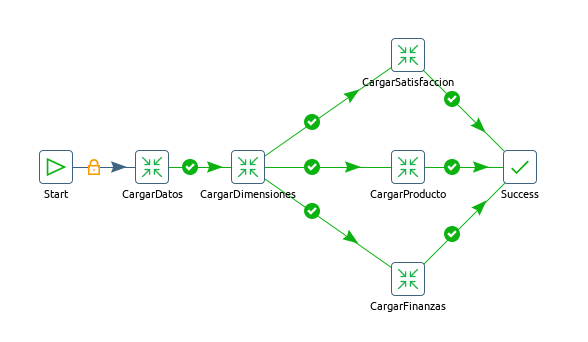
\includegraphics[width=0.7\textwidth]{fotos/ETL.png}
    \caption{Flujo principal del proceso ETL.}
    \label{fig:etl_principal}
\end{figure}

\subsection{Cargar Datos}

La transformación \textit{CargarDatos} extrae información económica contenida en los archivos XML generados por cada restaurante. Este flujo incluye los siguientes pasos principales (figura~\ref{fig:etl_datos}):

\begin{enumerate}
    \item \textbf{Obtención de Datos:} Procesamos los archivos XML para extraer información clave, como ingresos, gastos y número de clientes.
    \item \textbf{Ordenación y Agrupación:} Ordenamos y agrupamos los datos por restaurante y periodo (año y mes).
    \item \textbf{Inserción en la Base de Datos:} Insertamos los datos procesados en las tablas de hechos correspondientes en el almacén de datos.
\end{enumerate}

\begin{figure}[h]
    \centering
    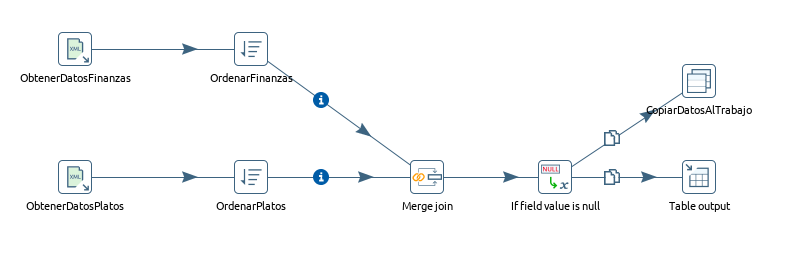
\includegraphics[width=0.8\textwidth]{fotos/CargarDatos.png}
    \caption{Flujo de pasos de la transformación \textit{CargarDatos}.}
    \label{fig:etl_datos}
\end{figure}

\subsection{Cargar Dimensiones}

La transformación \textbf{CargarDimensiones} se encarga de procesar los datos iniciales y crear las tablas correspondientes a las tres dimensiones requeridas: \textbf{Tiempo}, \textbf{Restaurante} y \textbf{Producto}. En el caso de la dimensión \textbf{Restaurante}, incorporamos dos mapeadores adicionales que vinculan el identificador del restaurante con su ciudad y país respectivos. \\

\begin{figure}[h]
    \centering
    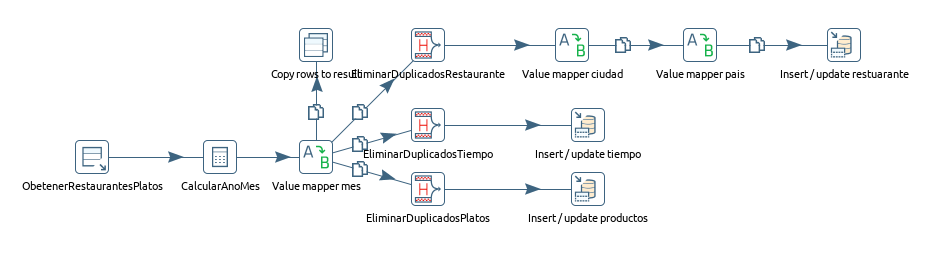
\includegraphics[width=0.9\textwidth]{fotos/CargarDimensiones.png}
    \caption{Flujo de pasos de la transformación \textit{CargarDimensiones}.}
    \label{fig:etl_cargardimensiones}
\end{figure}

\noindent Mostramos a continuación las dimensiones con los datos tras el proceso de carga:

\begin{figure}[H]
    \centering
    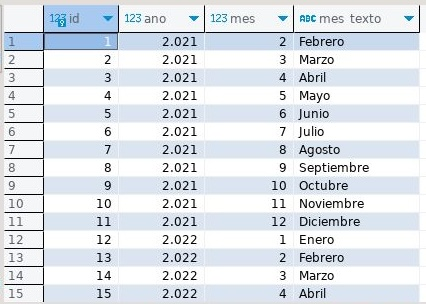
\includegraphics[width=0.35\textwidth]{fotos/dim_tiempo.jpg}
    \caption{Muestra de la dimensión \texttt{tiempo}.}
    \label{fig:dim1}
\end{figure}

\begin{figure}[H]
    \centering
    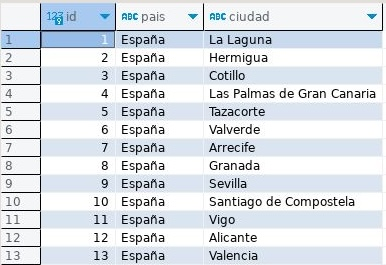
\includegraphics[width=0.35\textwidth]{fotos/dim_restaurante.jpg}
    \caption{Muestra de la dimensión \texttt{restaurante}.}
    \label{fig:dim2}
\end{figure}

\begin{figure}[H]
    \centering
    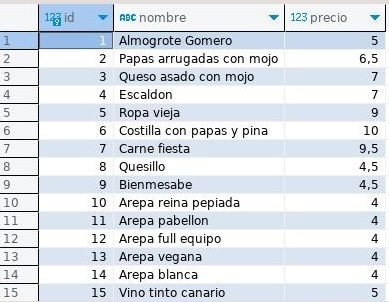
\includegraphics[width=0.35\textwidth]{fotos/dim_productos.jpg}
    \caption{Muestra de la dimensión \texttt{productos}.}
    \label{fig:dim3}
\end{figure}

\subsection{Cargar Valoraciones de Clientes}

La transformación \textit{CargarSatisfaccion} procesa las valoraciones de clientes contenidas en los archivos CSV generados por los restaurantes. Esta transformación sigue los pasos principales que detallamos a continuación (figura~\ref{fig:etl_valoraciones}):

\begin{enumerate}
    \item \textbf{Lectura de Archivos CSV:} Cargamos todos los archivos presentes en el directorio de trabajo que sigan el patrón de nombres indicado.
    \item \textbf{Unión de Datos:} Combinamos las valoraciones con los datos de los restaurantes utilizando un \textit{Database Join}.
    \item \textbf{Obtención de la referencia de fecha:} Mediante la fecha del reporte, obetenemos el mes y el año y consultamos a la base de datos cual es la refencia de fecha en la tabla de dimensión temporal.
    \item \textbf{Cálculo de Medidas:} Después de ordenar los datos, realizamos un agrupamiento (\textit{Group By} por restaurante, año y mes) de los siguientes campos:
    \begin{itemize}
        \item \texttt{valoracion\_ambiente} (media de la valoración del ambiente).
        \item \texttt{valoracion\_comida} (media de la valoración de la comida).
        \item \texttt{valoracion\_personal} (media de la valoración del personal).
    \end{itemize}
    \item \textbf{Inserción en la Base de Datos:} Insertamos los resultados procesados en las tablas de hechos correspondientes, añadiendo los siguientes campos:
    \begin{itemize}
        \item \texttt{restaurante}
        \item \texttt{fecha}
        \item \texttt{valoracion\_ambiente}
        \item \texttt{valoracion\_personal}
        \item \texttt{valoracion\_comida}
    \end{itemize}
\end{enumerate}

\begin{figure}[h]
    \centering
    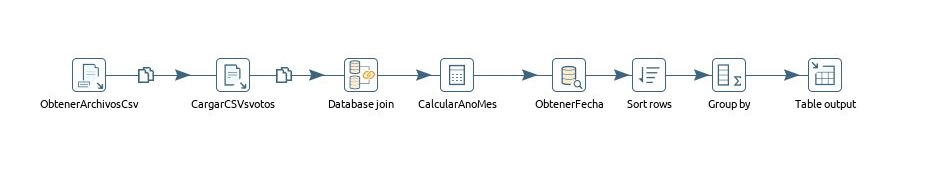
\includegraphics[width=0.8\textwidth]{fotos/cargarsatisfaccion.jpg}
    \caption{Flujo de pasos de la transformación \textit{CargarSatisfaccion}.}
    \label{fig:etl_valoraciones}
\end{figure}

\subsection{Cargar Productos}

La transformación \textit{CargarProductos} procesa los datos relacionados con los productos ofrecidos por cada restaurante a partir de los archivos XML. Durante esta transformación, extraemos información clave sobre los productos, como su identificador, nombre, número de ventas y precio. Además, ordenamos y agrupamos antes de calcular los ingresos generados por cada producto para cada restaurante y período. \\

\noindent Los datos que finalmente añadimos a la tabla de hechos de productos son los siguientes:

\begin{itemize}
    \item \texttt{restaurante}: Identificador único del restaurante.
    \item \texttt{fecha}: Año y mes, referenciados por id.
    \item \texttt{producto}: Identificador único del plato.
    \item \texttt{ventas}: Número total de ventas del plato.
    \item \texttt{ingresos}: Ingresos generados por el plato (\texttt{plato\_ventas} $\times$ \texttt{plato\_precio}).
\end{itemize}

\noindent El flujo de esta transformación lo mostramos en la figura~\ref{fig:etl_productos}.

\begin{figure}[h]
    \centering
    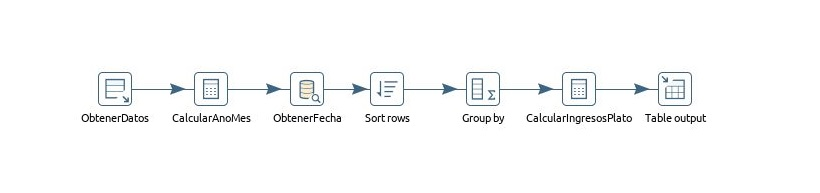
\includegraphics[width=0.8\textwidth]{fotos/cargarproducto.jpg}
    \caption{Flujo de pasos de la transformación \textit{CargarProductos}.}
    \label{fig:etl_productos}
\end{figure}

\subsection{Cargar Finanzas}

La transformación \textit{CargarFinanzas} procesa la información financiera extraída de los archivos XML y realiza cálculos adicionales basados en estos datos para enriquecer las tablas de hechos. Durante esta transformación, calculamos indicadores clave relacionados con la economía de los restaurantes, tales como porcentajes, ratios y métricas por cliente. \\

\noindent Los datos que finalmente añadimos a la tabla de hechos de finanzas incluyen los siguientes:

\begin{itemize}
    \item \texttt{id}: Identificador único del restaurante.
    \item \texttt{fecha}: Año y mes, referenciados por id y obtenidos a partir de la fecha del reporte.
    \item \texttt{alquiler}: Gasto en alquiler del restaurante.
    \item \texttt{proveedores}: Gasto en suministros.
    \item \texttt{personal}: Gasto personal.
    \item \texttt{extra}: Gasto en conceptos adicionales (limpieza, mantenimiento, etc.).
    \item \texttt{ingresos\_presencial}: Ingresos generados por ventas presenciales.
    \item \texttt{ingresos\_domicilio}: Ingresos generados por ventas a domicilio.
    \item \texttt{numero\_clientes\_presencial}: Cantidad total de clientes presenciales.
    \item \texttt{numero\_clientes\_domicilio}: Cantidad total de clientes del servicio a domicilio.
    \item \texttt{nuevos\_clientes\_presencial}: Nuevos clientes presenciales durante este mes.
    \item \texttt{nuevos\_clientes\_domicilio}: Nuevos clientes del servicio a domicilio durante este mes.
\end{itemize}

El flujo de esta transformación lo mostramos en la figura~\ref{fig:etl_finanzas}.

\begin{figure}[H]
    \centering
    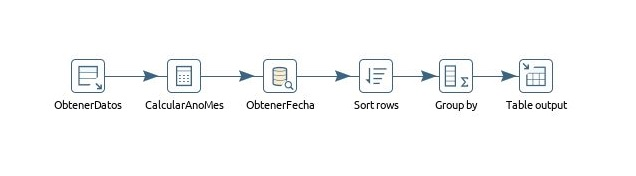
\includegraphics[width=0.8\textwidth]{fotos/cargasfinanzas.jpg}
    \caption{Flujo de pasos de la transformación \textit{CargarFinanzas}.}
    \label{fig:etl_finanzas}
\end{figure}

\subsection{Tablas de Hechos}

Hemos diseñado el almacén de datos para la cadena de restaurantes generando tres tablas de hechos principales, cada una asociada a un proceso de carga definido en el sistema ETL. Estas tablas almacenan datos relacionados con finanzas, productos y las valoraciones de los clientes. A continuación, describimos brevemente estas tablas:

\subsubsection{Hechos de Finanzas}

La tabla \texttt{finanzas} almacena datos económicos mensuales de cada restaurante. Esto nos permite evaluar la rentabilidad y el desempeño financiero tanto a nivel local como de toda la cadena. Una muestra de esta tabla puede verse en la figura~\ref{fig:tablahechos1}.

\begin{figure}[h]
    \centering
    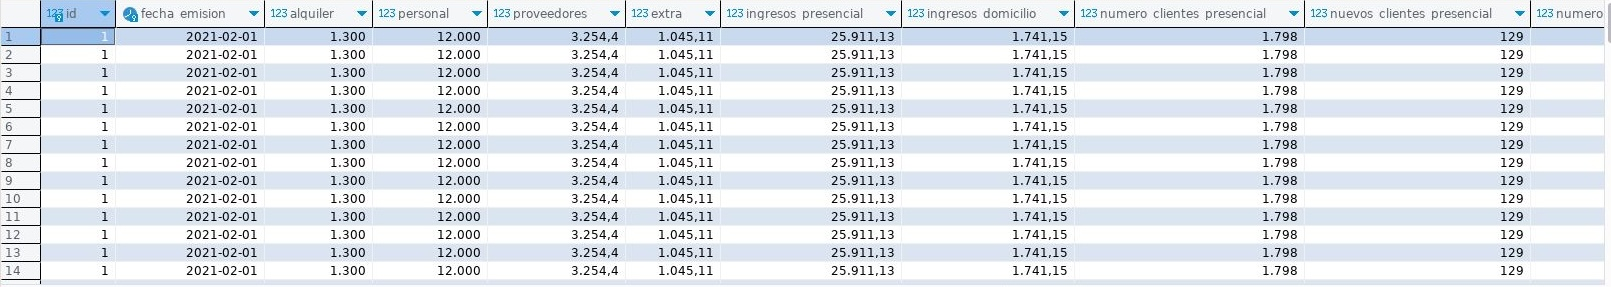
\includegraphics[width=0.9\textwidth]{fotos/etl_tabla_transitoria.jpg}
    \caption{Muestra de la tabla de hechos \texttt{finanzas}.}
    \label{fig:tablahechos1}
\end{figure}

\subsubsection{Hechos de Productos}

La tabla \texttt{productos} registra las ventas de cada plato ofrecido en los restaurantes, así como los ingresos asociados a estas ventas. Esto es fundamental para evaluar la popularidad de los productos y su contribución al ingreso total. La figura~\ref{fig:tablahechos2} presenta un ejemplo de los datos contenidos en esta tabla.

\begin{figure}[h]
    \centering
    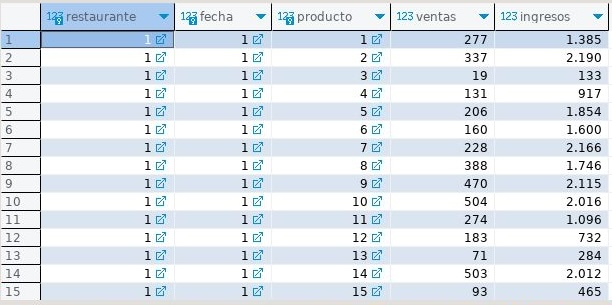
\includegraphics[width=0.55\textwidth]{fotos/fact_ventas.jpg}
    \caption{Muestra de la tabla de hechos \texttt{productos}.}
    \label{fig:tablahechos2}
\end{figure}
\newpage
\subsubsection{Hechos de Satisfacción de Usuarios}

La tabla \texttt{satisfacción\_usuarios} almacena las valoraciones de los clientes por local y periodo, tanto para consumo presencial como a domicilio. Incluye promedios de las valoraciones sobre ambiente, personal y calidad de la comida. En la figura~\ref{fig:tablahechos3} mostramos una vista de esta tabla.

\begin{figure}[h]
    \centering
    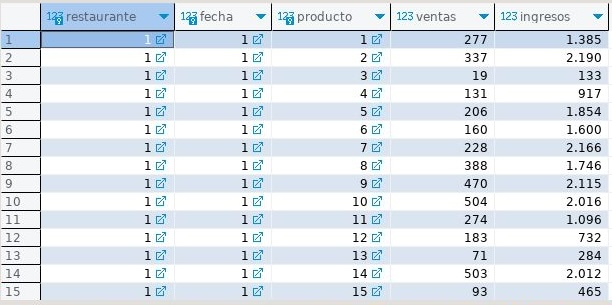
\includegraphics[width=0.55\textwidth]{fotos/fact_ventas.jpg}
    \caption{Muestra de la tabla de hechos \texttt{satisfacción\_usuarios}.}
    \label{fig:tablahechos3}
\end{figure}











\section{Análisis de datos con MDX y ROLAP}

Enfocaremos las consultas en gran medida en la búsqueda de patrones estacionales, tanto de beneficios o variables económicas como de satisfacción de los clientes. Como negocio de restauración, es probable que la demanda y la satisfacción de los clientes varíen a lo largo del año, por lo que es importante que identifiquemos estos patrones para poder anticiparnos y adaptar la oferta y el servicio en consecuencia.

\subsection{Consultas MDX}

Para ilustrar el uso de los cubos creados en la resolución de procesos de análisis se han resuelto las siguientes consultas usando el lenguaje MDX. Para cada consulta se proporciona su enunciado, el código MDX y una muestra del resultado.

\subsubsection{Muestra la evolución del número de clientes en el local de Las Palmas de Gran Canaria desde que hay registros.}

Esta consulta permite comprender la clientela del local de Las Palmas de Gran Canaria desde que se tienen registros. Nos permite diferenciar entre clientes presenciales y a domicilio, así como entre clientes nuevos y recurrentes. Con todo esto y, al representarlo frente al tiempo, podemos analizar la evolución, buscar patrones estacionales, etc.

\begin{lstlisting}[style=terminal]
WITH
SET [~Restaurante_Restaurante.jerarquiaRestaurantes_pais] AS
    Exists({[Restaurante.jerarquiaRestaurantes].[pais].Members}, [~Restaurante_Restaurante.jerarquiaRestaurantes_ciudad])
SET [~Restaurante_Restaurante.jerarquiaRestaurantes_ciudad] AS
    {[Restaurante.jerarquiaRestaurantes].[Espana].[Las Palmas de Gran Canaria]}
SET [~FILTER] AS
    [~Restaurante_Restaurante.jerarquiaRestaurantes_ciudad]
SET [~Tiempo_Tiempo.jerarquiaTiempo_ano] AS
    {[Tiempo.jerarquiaTiempo].[2023], [Tiempo.jerarquiaTiempo].[2022]}
SET [~Tiempo_Tiempo.jerarquiaTiempo_mes] AS
    Exists({[Tiempo.jerarquiaTiempo].[mes].Members}, [~Tiempo_Tiempo.jerarquiaTiempo_ano])
SET [~ROWS] AS
    Hierarchize({[~Tiempo_Tiempo.jerarquiaTiempo_ano], [~Tiempo_Tiempo.jerarquiaTiempo_mes]})
SELECT
NON EMPTY {[Measures].[Numero clientes presencial], [Measures].[Nuevos clientes domicilio], [Measures].[Numero clientes domicilio], [Measures].[Nuevos clientes presencial]} ON COLUMNS,
NON EMPTY [~ROWS] ON ROWS
FROM [Finanzas]
WHERE [~FILTER]
\end{lstlisting}

\begin{figure}[H]
    \centering
    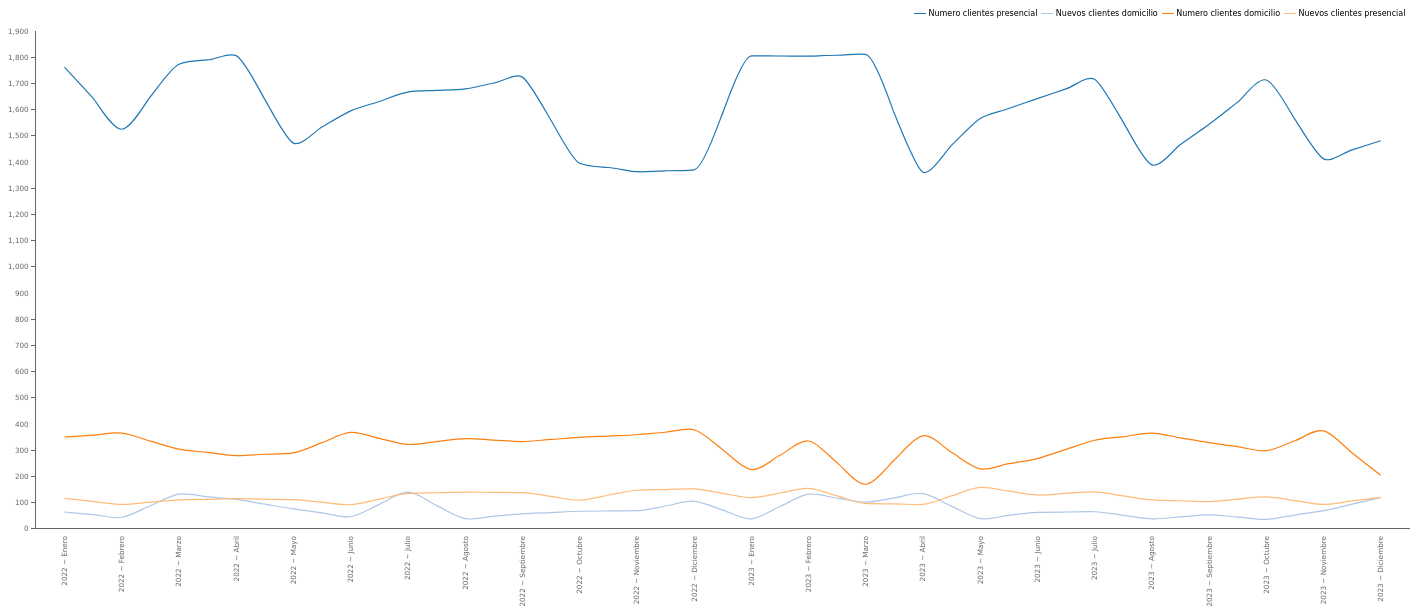
\includegraphics[width=\textwidth]{fotos/clientesLasPalmas.png}
    \caption{Evolución en el número de clientes Las Palmas de Gran Canaria desde 2021.}
    \label{fig:consulta3}
\end{figure}

\subsubsection{Muestra la satisfacción media en cada local a principio y a finales de cada año de los que se tienen registros.}

Esta consulta nos permite comparar la satisfacción media de los clientes en cada local a principio y finales de año. Esto puede ser útil para identificar posibles patrones estacionales en la satisfacción de los clientes, así como para evaluar la evolución de la calidad del servicio, comparando principio y final de año.

\begin{lstlisting}[style=terminal]
WITH
SET [~COLUMNS] AS
    {[Restaurante.jerarquiaRestaurantes].[ciudad].Members}
MEMBER [Measures].[valoracion_media] AS
    ((([Measures].[Valoracion personal] + [Measures].[Valoracion ambiente]) + [Measures].[Valoracion comida]) / 3), FORMAT_STRING = "#,##0.00"
SET [~Tiempo_Tiempo.jerarquiaTiempo_ano] AS
    Exists({[Tiempo.jerarquiaTiempo].[ano].Members}, [~Tiempo_Tiempo.jerarquiaTiempo_mes])
SET [~Tiempo_Tiempo.jerarquiaTiempo_mes] AS
    {[Tiempo.jerarquiaTiempo].[2022].[Enero], [Tiempo.jerarquiaTiempo].[2023].[Enero], [Tiempo.jerarquiaTiempo].[2024].[Enero], [Tiempo.jerarquiaTiempo].[2021].[Diciembre], [Tiempo.jerarquiaTiempo].[2022].[Diciembre], [Tiempo.jerarquiaTiempo].[2023].[Diciembre]}
SET [~ROWS] AS
    Hierarchize({[~Tiempo_Tiempo.jerarquiaTiempo_ano], [~Tiempo_Tiempo.jerarquiaTiempo_mes]})
SELECT
NON EMPTY CrossJoin([~COLUMNS], {[Measures].[valoracion_media]}) ON COLUMNS,
NON EMPTY [~ROWS] ON ROWS
FROM [Feedback]
\end{lstlisting}

\begin{figure}[H]
    \centering
    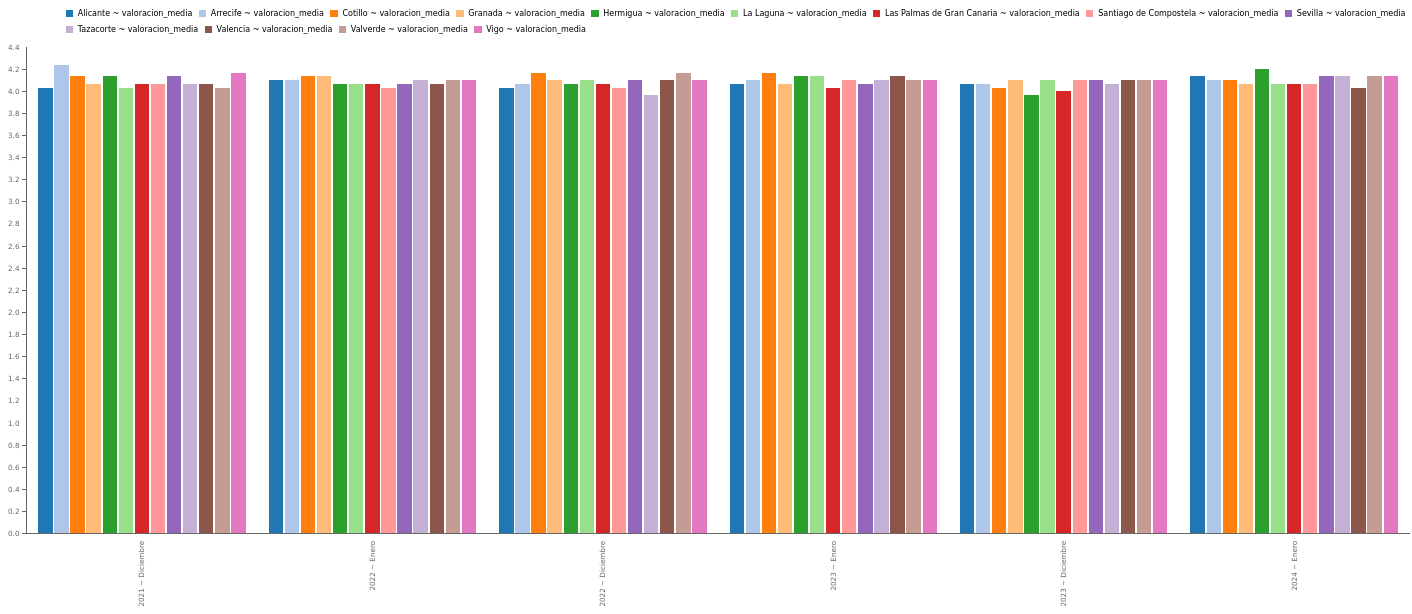
\includegraphics[width=\textwidth]{fotos/valoracionMediaEneroDiciembre.png}
    \caption{Satisfacción media a principio y finales de año en cada local.}
    \label{fig:consulta5}
\end{figure}

\subsubsection{Muestra, para todos los locales y para cada mes y año del que tengan registros, los ingresos totales frente a los gastos totales.}

Esta consulta nos permite comparar los ingresos totales frente a los gastos totales de cada local para cada mes y año del que se tienen registros. Esto es útil para evaluar la rentabilidad de cada local, identificar cuantitativamente posibles patrones estacionales en los ingresos y gastos, y comparar la evolución de los ingresos y gastos a lo largo del tiempo.

\begin{lstlisting}[style=terminal]
WITH
SET [~COLUMNS] AS
    {[Restaurante.jerarquiaRestaurantes].[ciudad].Members}
SET [~ROWS] AS
    Hierarchize({{[Tiempo.jerarquiaTiempo].[ano].Members}, {[Tiempo.jerarquiaTiempo].[mes].Members}})
SELECT
NON EMPTY CrossJoin([~COLUMNS], {[Measures].[Ingresos totales], [Measures].[Gastos totales]}) ON COLUMNS,
NON EMPTY [~ROWS] ON ROWS
FROM [Finanzas]
\end{lstlisting}

\begin{figure}[H]
    \centering
    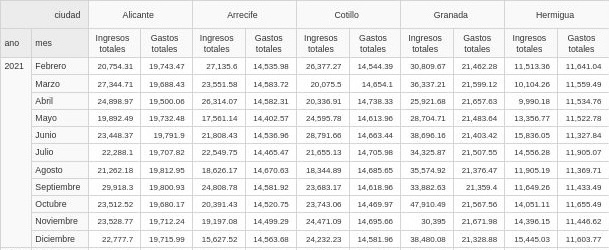
\includegraphics[width=0.8\textwidth]{fotos/ingresos_gastos.jpg}
    \caption{Ingresos y gastos de cada local.}
    \label{fig:consulta4}
\end{figure}


\subsubsection{Muestra el beneficio frente al número de clientes de cada restaurante.}

Esta consulta nos permite comparar el beneficio frente al número de clientes de cada restaurante. Esto es útil para evaluar la rentabilidad de cada local en función de su clientela, identificar posibles patrones en la relación entre beneficio y número de clientes, y comparar la rentabilidad de los locales en función de su clientela general.


\begin{lstlisting}[style=terminal]
WITH
SET [~ROWS] AS
    {[Restaurante.jerarquiaRestaurantes].[ciudad].Members}
SELECT
NON EMPTY {[Measures].[Beneficio], [Measures].[Numero clientes]} ON COLUMNS,
NON EMPTY [~ROWS] ON ROWS
FROM [Finanzas]
\end{lstlisting}

\begin{figure}[H]
    \centering
    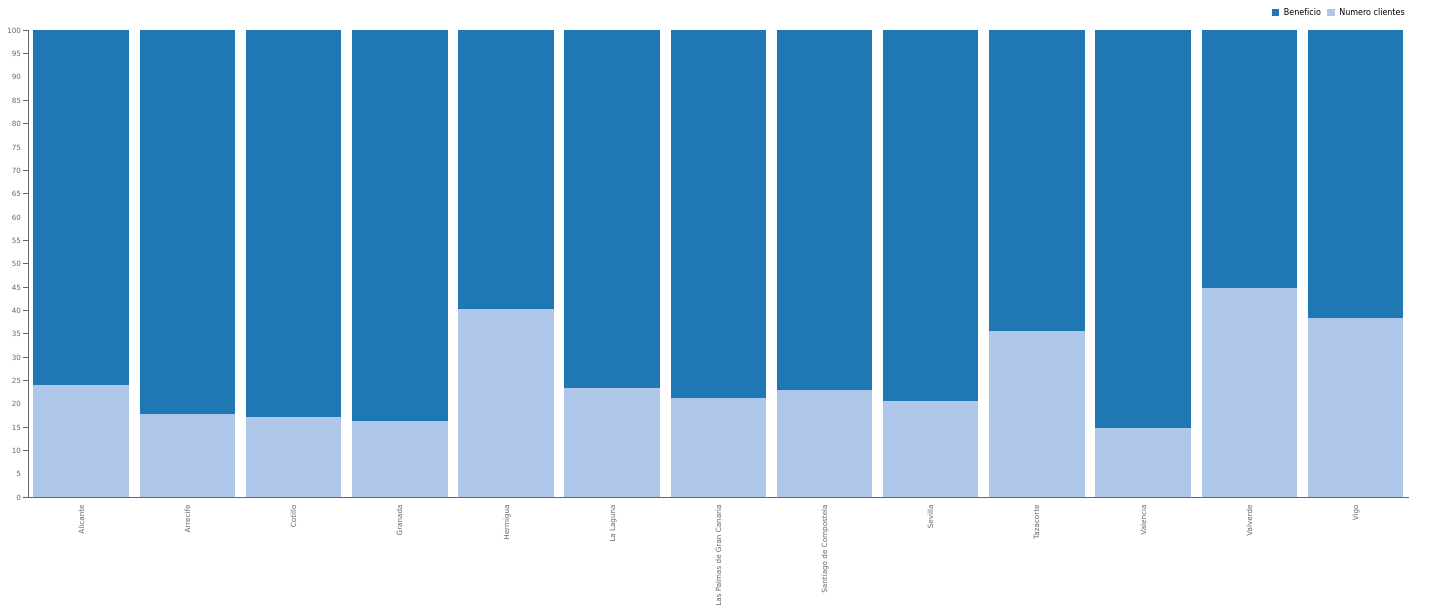
\includegraphics[width=\textwidth]{fotos/beneficioVsCliente.png}
    \caption{Beneficio frente al número de neuvos clientes.}
    \label{fig:consulta2}
\end{figure}









\subsection{Consultas ROLAP}

Con las siguientes consultas ilustramos el uso de la extensión del SQL para OLAP para solucionar problemas de análisis.

\subsubsection{Ranking de productos más vendidos por restaurante, basado en el número de ventas totales.}

Esta consulta nos permite identificar los productos más vendidos en cada local, basándonos en el número total de ventas. Esto es útil para identificar los productos más populares en cada local, evaluar la rentabilidad de cada producto y comparar la popularidad de los productos en diferentes locales.

\begin{lstlisting}[style=sql]
SELECT 
    r.ciudad  AS ciudad,
    p.nombre AS producto,
    SUM(v.ventas) AS total_ventas,
    RANK() OVER (PARTITION BY r.id ORDER BY SUM(v.ventas) DESC) AS ranking_producto
FROM 
    fact_ventas v
JOIN 
    dim_restaurante r ON v.restaurante = r.id
JOIN 
    dim_productos p ON v.producto = p.id
GROUP BY 
    r.id, p.nombre
ORDER BY 
    r.id, ranking_producto;
\end{lstlisting}

\begin{figure}[H]
    \centering
    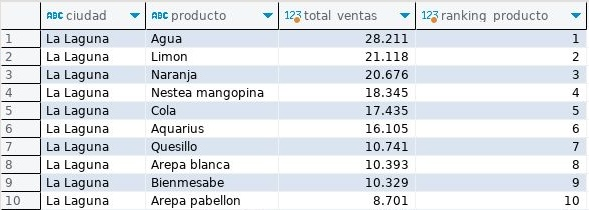
\includegraphics[width=0.7\textwidth]{fotos/q2.jpg}
    \caption{Productos más vendidos en el local de La Laguna.}
    \label{fig:rolap1}
\end{figure}


\subsubsection{Calcula la variación porcentual mensual de los ingresos presenciales por restaurante.}

Esta consulta nos permite calcular la variación porcentual mensual de los ingresos presenciales por restaurante. Esto es útil para evaluar la evolución de los ingresos presenciales de cada local, identificar posibles patrones estacionales en los ingresos y comparar la evolución de los ingresos presenciales de los locales a lo largo del tiempo.


\begin{lstlisting}[style=sql]
SELECT 
    r.ciudad AS ciudad,
    t.ano,
    t.mes_texto AS mes,
    SUM(f.ingresos_presencial) AS ingresos_mes,
    LAG(SUM(f.ingresos_presencial)) OVER (PARTITION BY r.id ORDER BY t.ano, t.mes) AS ingresos_mes_anterior,
    CASE 
        WHEN LAG(SUM(f.ingresos_presencial)) OVER (PARTITION BY r.id ORDER BY t.ano, t.mes) IS NULL THEN NULL
        ELSE ROUND(
            (SUM(f.ingresos_presencial) - LAG(SUM(f.ingresos_presencial)) OVER (PARTITION BY r.id ORDER BY t.ano, t.mes)) 
            / LAG(SUM(f.ingresos_presencial)) OVER (PARTITION BY r.id ORDER BY t.ano, t.mes) * 100, 2)
    END AS variacion_porcentual
FROM 
    fact_finanzas f
JOIN 
    dim_restaurante r ON f.restaurante = r.id
JOIN 
    dim_tiempo t ON f.fecha = t.id
GROUP BY 
    r.id, r.ciudad, t.ano, t.mes, t.mes_texto
ORDER BY 
    r.ciudad, t.ano, t.mes;
\end{lstlisting}

\begin{figure}[H]
    \centering
    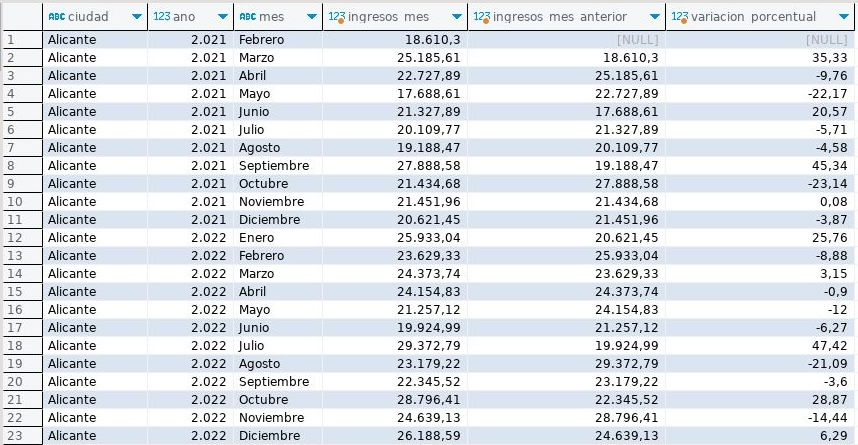
\includegraphics[width=0.7\textwidth]{fotos/q3.jpg}
    \caption{Variación mensual porcentual de los ingresos presenciales por restaurante.}
    \label{fig:rolap2}
\end{figure}


\subsubsection{Calcular una media móvil de tres meses para las valoraciones del restaurante.}

Esta consulta nos permite calcular una media móvil de tres meses para las valoraciones de cada restaurante. Esto es útil para suavizar las fluctuaciones en las valoraciones de los clientes, identificar tendencias a largo plazo en la satisfacción de los clientes y comparar la evolución de las valoraciones de los restaurantes a lo largo del tiempo.

\begin{lstlisting}[style=terminal]
SELECT 
    r.ciudad AS ciudad,
    t.ano,
    t.mes,
    f.valoracion_ambiente,
    f.valoracion_personal,
    f.valoracion_comida,
    ROUND(
        (f.valoracion_ambiente + f.valoracion_personal + f.valoracion_comida) / 3.0, 2
    ) AS valoracion_total,
    ROUND(
        AVG((f.valoracion_ambiente + f.valoracion_personal + f.valoracion_comida) / 3.0) OVER (
            PARTITION BY r.ciudad, r.id ORDER BY t.ano, t.mes ROWS BETWEEN 2 PRECEDING AND CURRENT ROW
        ), 2
    ) AS media_movil_3_meses
FROM 
    fact_satisfaccion f
JOIN 
    dim_restaurante r ON f.restaurante = r.id
JOIN 
    dim_tiempo t ON f.fecha = t.id
ORDER BY 
    r.ciudad, r.id, t.ano, t.mes;
\end{lstlisting}

\begin{figure}[H]
    \centering
    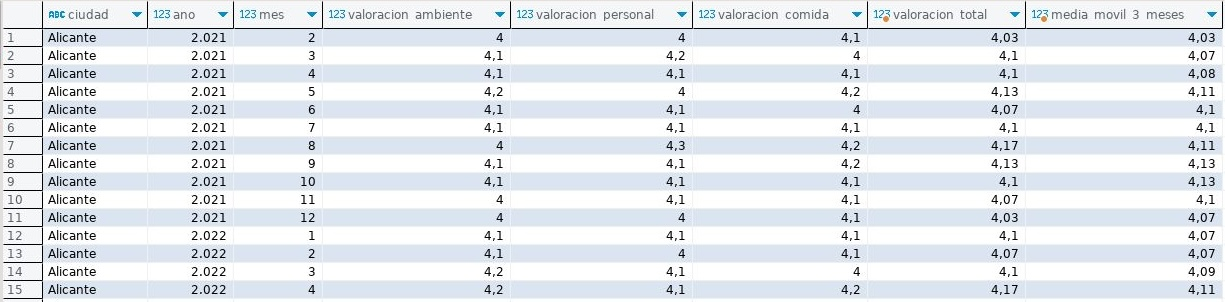
\includegraphics[width=\textwidth]{fotos/q4.jpg}
    \caption{Media móvil de tres meses para las valaraciones de cada restaurante.}
    \label{fig:rolap3}
\end{figure}


\subsubsection{Calcula el percentil de cada restaurante en términos de ingresos totales (presenciales + domicilio).}

Esta consulta nos permite calcular el percentil de cada restaurante en términos de ingresos totales (presenciales + domicilio). Esto es útil para evaluar la posición de cada restaurante en términos de ingresos totales, identificar los restaurantes más rentables y comparar la rentabilidad de los restaurantes en función de sus ingresos totales.

\begin{lstlisting}[style=terminal]
WITH ingresos_anuales AS (
    SELECT 
        r.ciudad AS ciudad,
        SUM(f.ingresos_presencial + f.ingresos_domicilio) AS ingresos_totales_anuales
    FROM 
        fact_finanzas f
    JOIN 
        dim_restaurante r ON f.restaurante = r.id
    JOIN 
        dim_tiempo t ON f.fecha = t.id
    GROUP BY 
        r.ciudad
)
SELECT 
    ciudad,
    ingresos_totales_anuales,
    ROUND(PERCENT_RANK() OVER (ORDER BY ingresos_totales_anuales DESC)::numeric * 100, 2) AS percentil
FROM 
    ingresos_anuales
ORDER BY 
    percentil;
\end{lstlisting}

\begin{figure}[H]
    \centering
    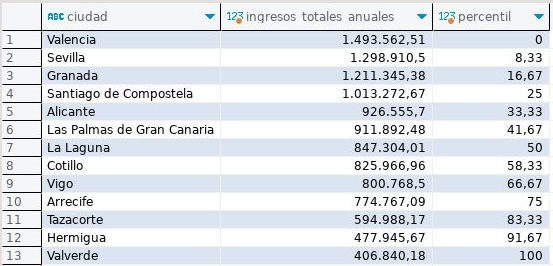
\includegraphics[width=0.7\textwidth]{fotos/q5.jpg}
    \caption{Percentil de cada restaurante según sus ingresos totales.}
    \label{fig:rolap4}
\end{figure}

\subsubsection{Identifica el porcentaje de nuevos clientes respecto al total por mes y restaurante.}

Esta consulta nos permite identificar el porcentaje de nuevos clientes respecto al total por mes y restaurante. Esto es útil para evaluar la proporción de nuevos clientes en cada restaurante, identificar posibles patrones estacionales en la llegada de nuevos clientes y comparar la evolución de los nuevos clientes en los restaurantes a lo largo del tiempo.

\begin{lstlisting}[style=terminal]
SELECT 
    r.ciudad AS ciudad,
    t.ano,
    t.mes,
    SUM(f.nuevos_clientes_presencial + f.nuevos_clientes_domicilio) AS nuevos_clientes,
    SUM(f.numero_clientes_presencial + f.numero_clientes_domicilio) AS total_clientes,
    ROUND(
        SUM(f.nuevos_clientes_presencial + f.nuevos_clientes_domicilio) * 100.0 
        / SUM(f.numero_clientes_presencial + f.numero_clientes_domicilio), 2
    ) AS porcentaje_nuevos_clientes
FROM 
    fact_finanzas f
JOIN 
    dim_restaurante r ON f.restaurante = r.id
JOIN 
    dim_tiempo t ON f.fecha = t.id
GROUP BY 
    r.ciudad, t.ano, t.mes
ORDER BY 
    r.ciudad, t.ano, t.mes;
\end{lstlisting}

\begin{figure}[H]
    \centering
    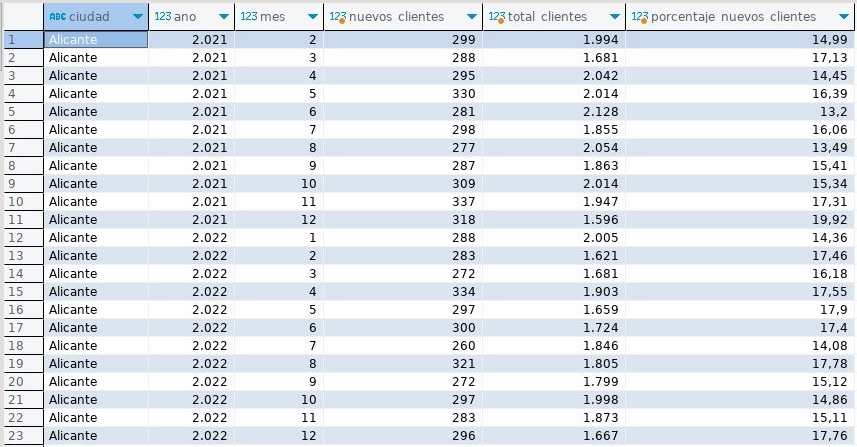
\includegraphics[width=0.7\textwidth]{fotos/q6.jpg}
    \caption{Porcentaje de nuevos clientes respecto al total por mes y restaurante.}
    \label{fig:rolap5}
\end{figure}




\section{Cuadro de mando e informe}

\noindent En esta sección se muestra un cuadro de mando y un informe generados con las herramientas de Pentaho.

\subsection{Cuadro de mando}

El cuadro de mando tiene como objetivo transmitir una visión global del estado de los diferentes restaurantes, tanto a nivel financiero como de valoración de los usuarios. Además, añadimos una gráfica que muestra los ingresos frente a la cantidad de usuarios de forma proporcional, lo cual nos permite comparar la eficiencia de las distintas franquicias a la hora de convertir clientes en beneficio. Todo esto lo podremos filtrar para un año de interés. Además, podremos filtrar por restaurante y por año para ver los platos estrella de cada lugar, posicionados por la cantidad de ingresos. \\

Todo esto nos permitirá tener la visión global que comentábamos antes, pero también poder ver en detalle qué platos son los que más ingresos generan en cada local. A continuación, dejamos varias vistas del cuadro de mando implementado:

\begin{figure}[H]
    \centering
    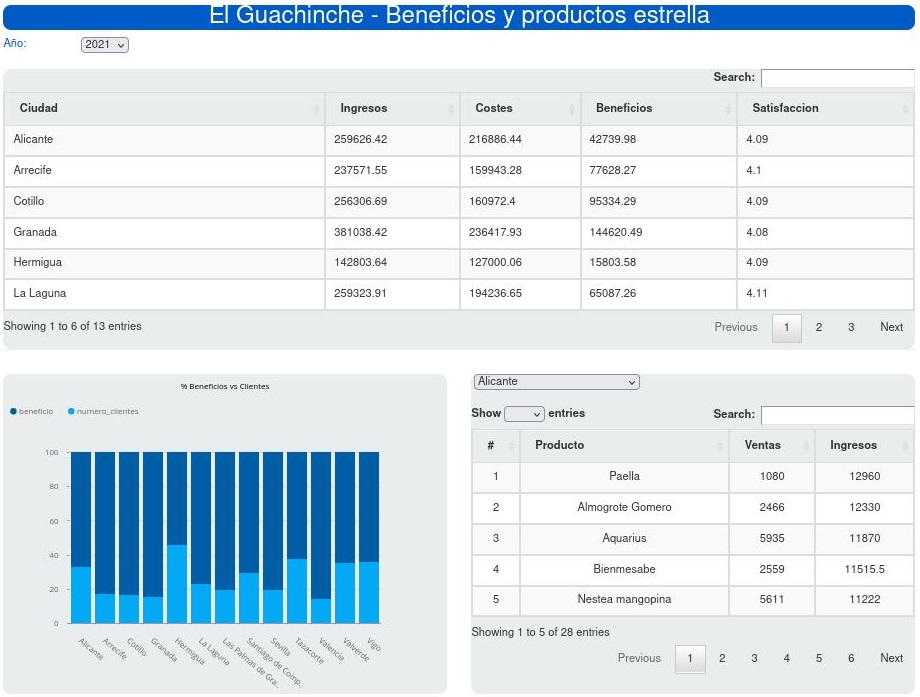
\includegraphics[height=0.44\textheight]{fotos/cuadro/cuadro_blanco.jpg}
    \caption{Cuadro de mando para los beneficios y productos estrella de los locales de El Guachinche. El panel de abajo a la derecha filtra resultados para el local de Alicante.}
    \label{fig:cuadro-blanco}
\end{figure}


\begin{figure}[H]
    \centering
    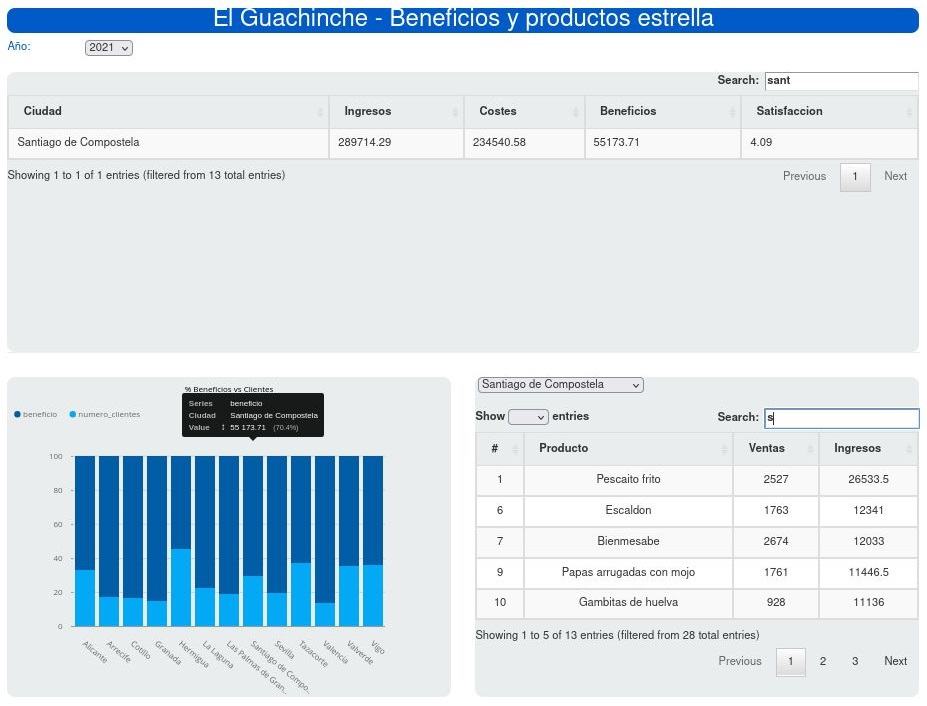
\includegraphics[height=0.44\textheight]{fotos/cuadro/2021-santiago.jpg}
    \caption{Datos relativos al local de Santiago de Compostela en el año 2021.}
    \label{fig:cuadro-santiago}
\end{figure}

\begin{figure}[H]
    \centering
    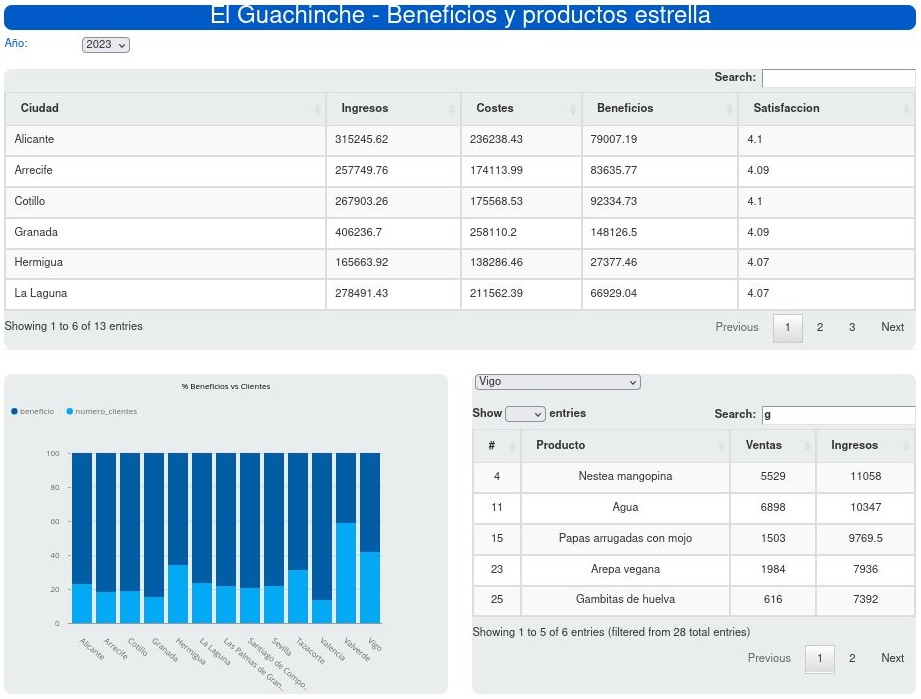
\includegraphics[height=0.44\textheight]{fotos/cuadro/2023-vigo-g.jpg}
    \caption{Datos relativos al local de Vigo en el año 2023.}
    \label{fig:cuadro-vigo}
\end{figure}

\subsection{Informe. Reporte financiero por ciudad}

El \textit{Reporte de Finanzas por Ciudad} presenta un análisis detallado del desempeño económico de la cadena de restaurantes \textbf{El Guachinche} durante el año 2023. Este informe se organiza por ciudades, proporcionando un desglose mensual de los siguientes indicadores clave:

\begin{itemize}
    \item \textbf{Ingresos:} Total de ventas generadas en cada mes.
    \item \textbf{Costes:} Gastos operativos asociados al funcionamiento de los restaurantes.
    \item \textbf{Beneficios:} Diferencia entre ingresos y costes, reflejando la rentabilidad mensual.
\end{itemize}

Cada sección del informe concluye con un resumen anual consolidado, lo que facilita la comparación del desempeño financiero entre las distintas ubicaciones. Este análisis es esencial para identificar:
\begin{itemize}
    \item Ciudades más rentables dentro de la cadena.
    \item Áreas con oportunidades para optimizar costos o mejorar márgenes de beneficio.
\end{itemize}

A continuación, y para finalizar el documento, se incluye el informe completo a modo de anexo, comenzando en la siguiente página.


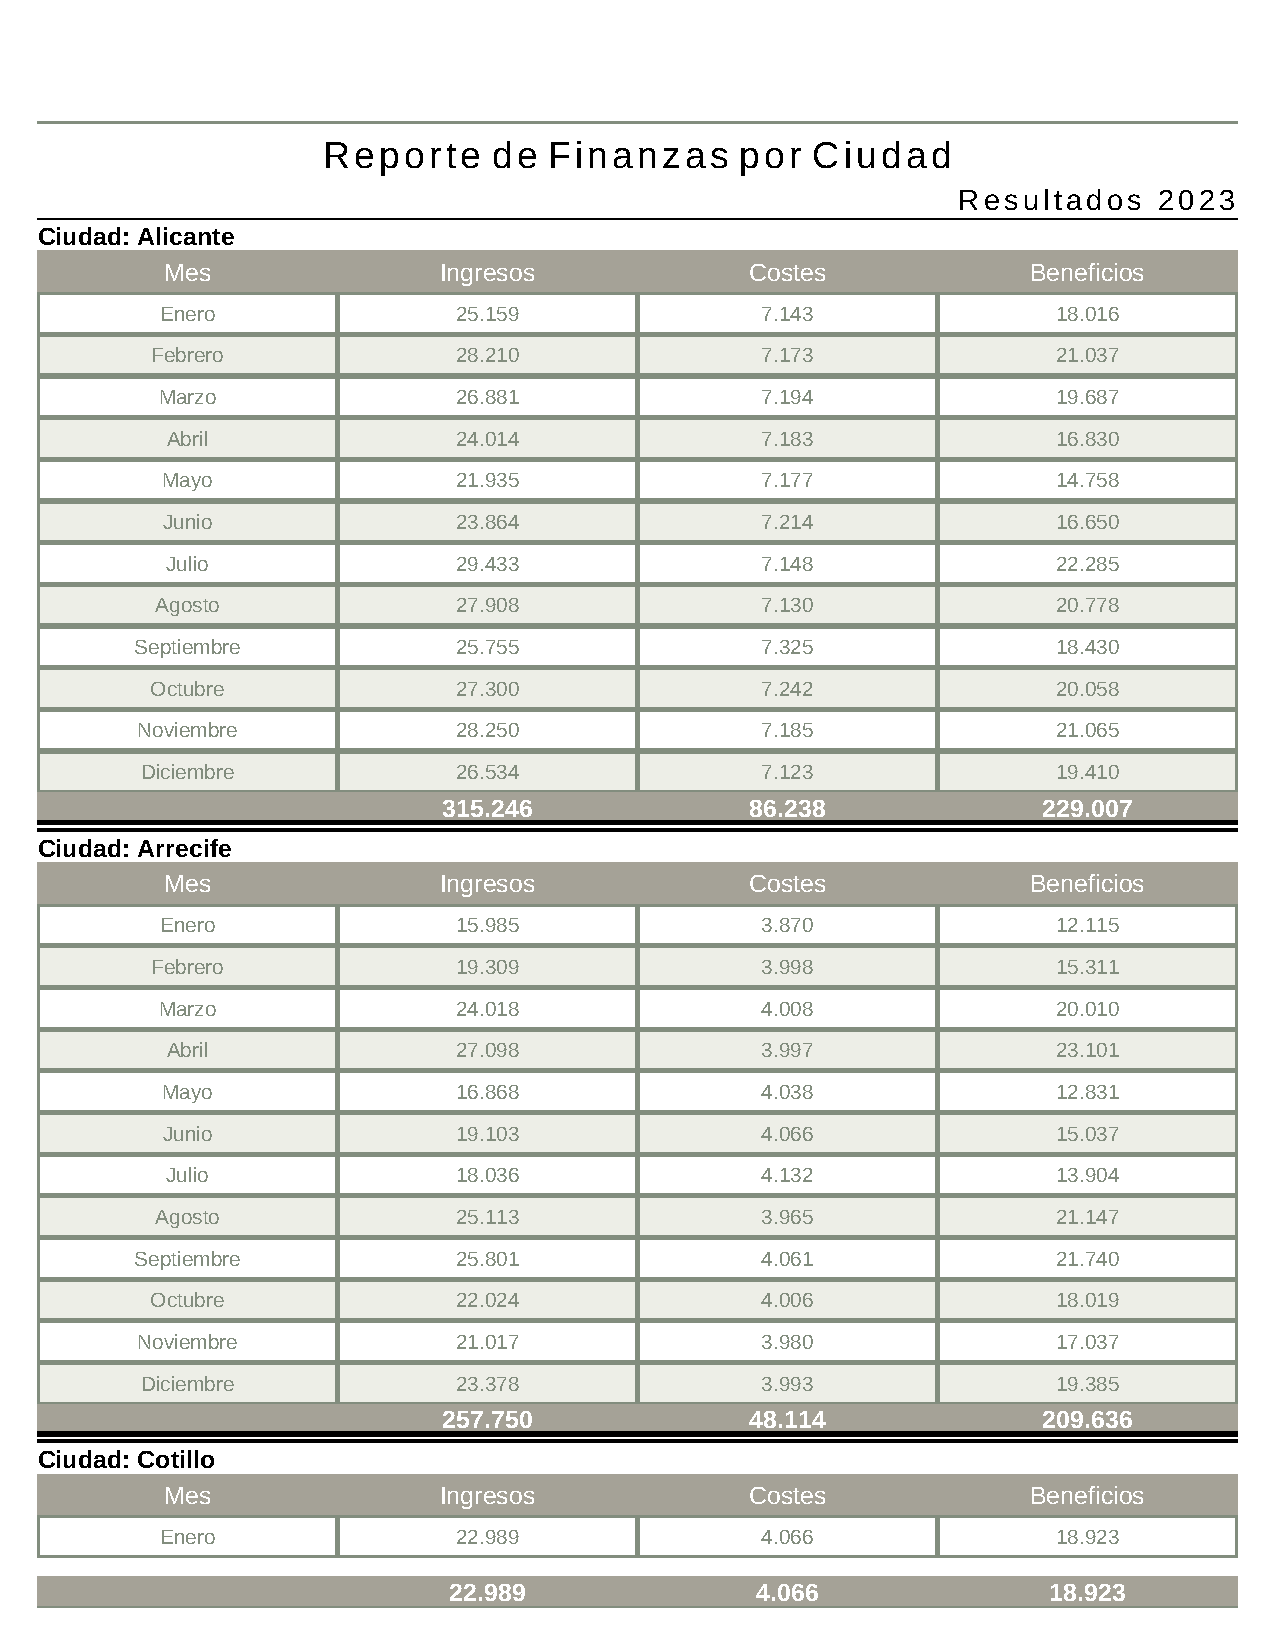
\includepdf[pages=-]{Reporte_finanzas_el_guachinche.pdf}

\end{document}

    